\chapter{Physical Design}

In this chapter we will study the \texttt{EXPLAIN PLAN} of the operations implemented to see if there is the need to define new indexes.

\subsection*{Operation 1 (10 times per day)}
\begin{figure}[H]
    \centering
    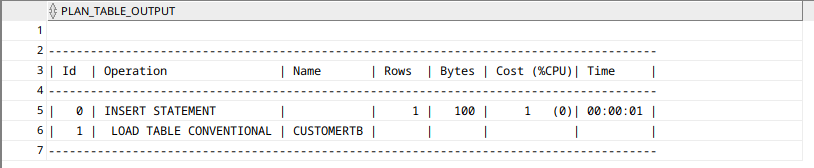
\includegraphics[width=0.8\textwidth]{img/phys/op1-1.png}
\end{figure}

\subsubsection*{Considerations}
The first query is a simple insert, so we don't need to optimize anything.

\subsection*{Operation 2 (1000 times per day)}
Operation 2 is composed of 2 queries, the first that retrieve the business account and the second that add the order.
\subsubsection*{First query}
\begin{figure}[H]
    \centering
    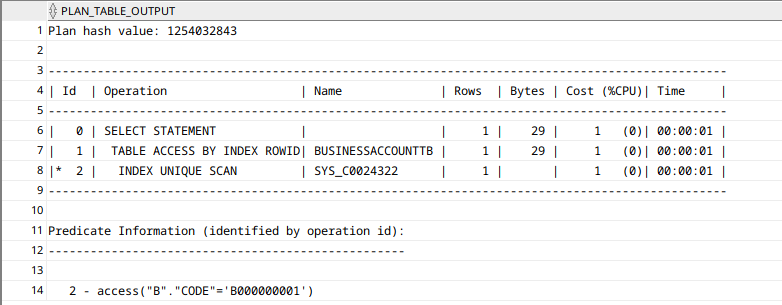
\includegraphics[width=0.8\textwidth]{img/phys/op2-1.png}
\end{figure}
\begin{figure}[H]
    \centering
    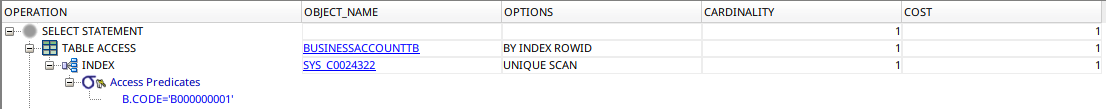
\includegraphics[width=0.8\textwidth]{img/phys/op2-3.png}
\end{figure}

\subsubsection*{Second query}
\begin{figure}[H]
    \centering
    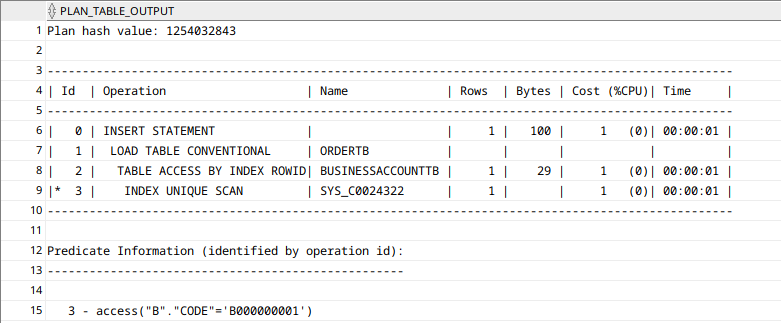
\includegraphics[width=0.8\textwidth]{img/phys/op2-2.png}
\end{figure}
\begin{figure}[H]
    \centering
    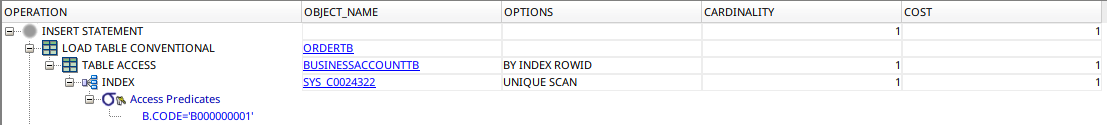
\includegraphics[width=0.8\textwidth]{img/phys/op2-4.png}
\end{figure}

\subsubsection*{Considerations}
The first query retrieves the business account from a key value, so it's already indexed. The second query is an insert, so we don't need to optimize anything.

\subsection*{Operation 3 (500 times per day)}
\begin{figure}[H]
    \centering
    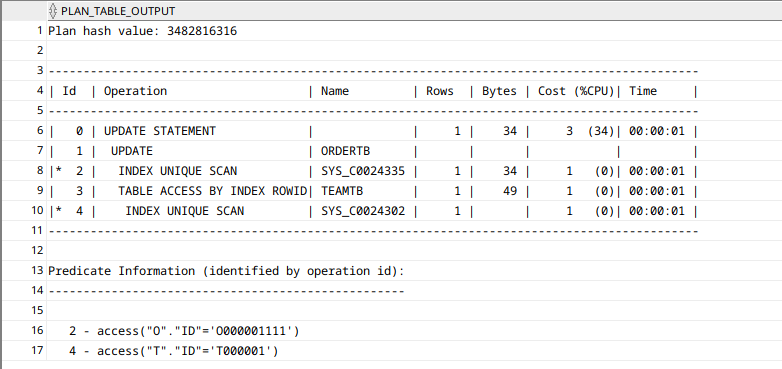
\includegraphics[width=0.8\textwidth]{img/phys/op3-1.png}
\end{figure}
\begin{figure}[H]
    \centering
    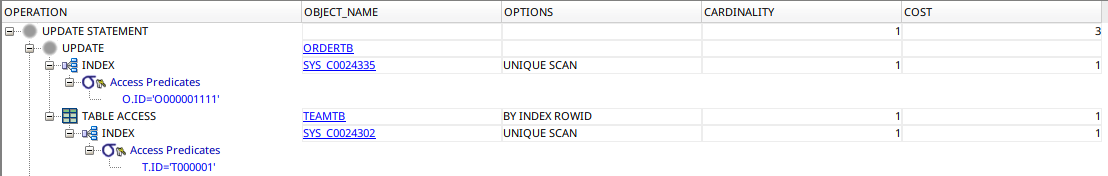
\includegraphics[width=0.8\textwidth]{img/phys/op3-2.png}
\end{figure}
\subsubsection*{Considerations}
The query is a simple update with punctual selection on a key value, so we don't need to optimize anything.

\subsection*{Operation 4A (200 times per day)}
\begin{figure}[H]
    \centering
    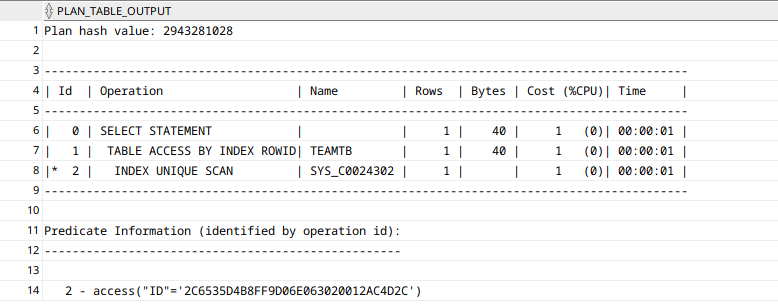
\includegraphics[width=0.8\textwidth]{img/phys/op4A-1.png}
\end{figure}
\begin{figure}[H]
    \centering
    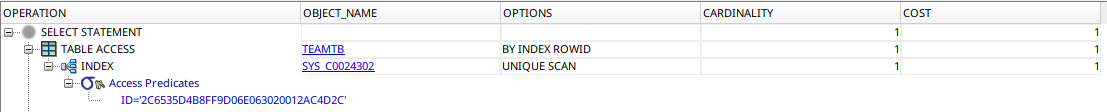
\includegraphics[width=0.8\textwidth]{img/phys/op4A-2.png}
\end{figure}
\subsubsection*{Considerations}
The query is a select with a punctual selection on a key value, so we don't need to optimize anything.

\subsection*{Operation 4B (200 times per day)}
\begin{figure}[H]
    \centering
    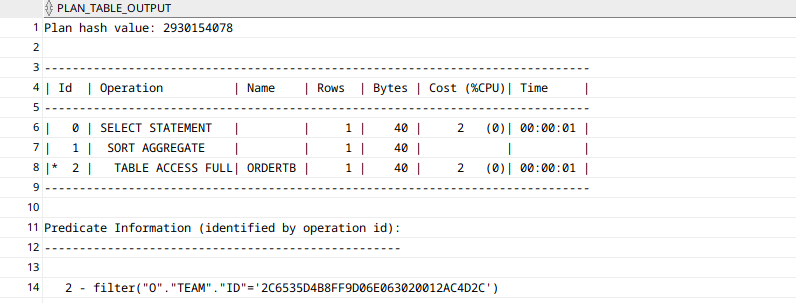
\includegraphics[width=0.8\textwidth]{img/phys/op4B-1.png}
\end{figure}
\begin{figure}[H]
    \centering
    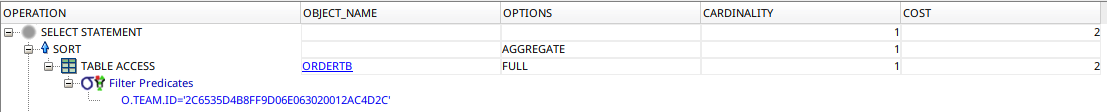
\includegraphics[width=0.8\textwidth]{img/phys/op4B-2.png}
\end{figure}
\subsubsection*{Considerations}
The query is a select with a punctual selection on a key value, with a full table scan given by the \textit{sum} function, but given the selection of a specific team on the basis of its key value, we don't need to optimize anything.

\subsection*{Operation 5 (20 times per day)}
\begin{figure}[H]
    \centering
    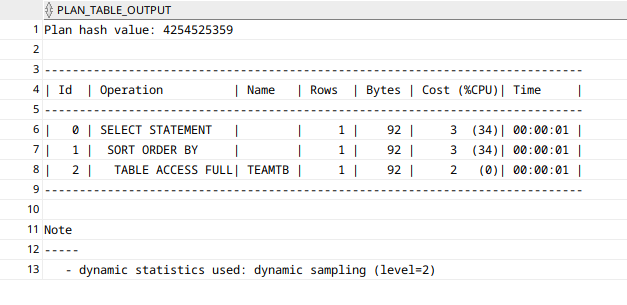
\includegraphics[width=0.8\textwidth]{img/phys/op5-1.png}
\end{figure}
\begin{figure}[H]
    \centering
    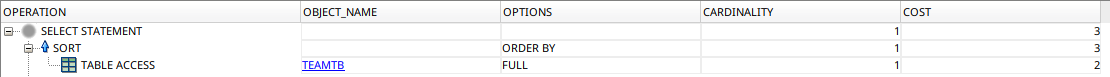
\includegraphics[width=0.8\textwidth]{img/phys/op5-2.png}
\end{figure}
\subsubsection*{Considerations}
The query needs to scan all the table \texttt{TeamTB} anyway, and \texttt{performanceScore} has duplicates, so we don't optimize.
